\documentclass[11pt]{article}
\usepackage{notes}
\definecolor{AccN}{HTML}{1E7A45}
\begin{document}
\titlepg{2}{Supervised Learning Part 1:\\Classification Algorithms}{Logistic regression, kNN, decision trees, random forests, boosting, SVMs and Naive Bayes --- applied to IADS threat classification}
\tableofcontents
\newpage

\section{The Classification Problem and the IADS Case Study}
\subsection{What classification is}
\begin{definition}{classification}
Given labelled training examples $D=\{(x_i,y_i)\}_{i=1}^N$ with feature vectors $x_i\in\mathbb R^d$ and labels $y_i$ from a finite set of $C$ classes, learn a function $f:\mathbb R^d\to\{1,\ldots,C\}$ that predicts the class of new, unseen examples. Most classifiers also output class probabilities $P(y=c\mid x)$, which allow thresholds to be set according to the cost of each error.
\end{definition}
Every classifier partitions feature space into regions, one per class. The surfaces separating these regions are the \textbf{decision boundaries}. Different algorithms produce boundaries of different shapes, which is why no single algorithm is best for every problem.
\begin{center}\resizebox{\textwidth}{!}{\begin{tikzpicture}[x=0.9cm,y=0.9cm]
\begin{scope}\draw[GreyN](0,0)rectangle(4,3);\foreach \x/\y in {0.4/2.4,0.9/2.0,0.6/1.5,1.2/2.6,1.5/1.8,1.0/1.0}{\fill[BluN](\x,\y)circle(0.07);}\foreach \x/\y in {2.6/0.5,3.1/1.1,2.4/1.3,3.4/0.6,2.8/1.7,3.3/2.0}{\fill[RedN](\x,\y)circle(0.07);}\draw[AccN,thick](1.4,0)--(2.2,3);\node[font=\scriptsize]at(2,-0.35){logistic: hyperplane};\end{scope}
\begin{scope}[xshift=4.4cm]\draw[GreyN](0,0)rectangle(4,3);\foreach \x/\y in {0.4/2.4,0.9/2.0,0.6/1.5,1.2/2.6,1.5/1.8,1.0/1.0}{\fill[BluN](\x,\y)circle(0.07);}\foreach \x/\y in {2.6/0.5,3.1/1.1,2.4/1.3,3.4/0.6,2.8/1.7,3.3/2.0}{\fill[RedN](\x,\y)circle(0.07);}\draw[AccN,thick](1.9,0)--(1.7,1.0)--(2.3,1.5)--(1.9,2.3)--(2.1,3);\node[font=\scriptsize]at(2,-0.35){kNN: piecewise, local};\end{scope}
\begin{scope}[xshift=8.8cm]\draw[GreyN](0,0)rectangle(4,3);\foreach \x/\y in {0.4/2.4,0.9/2.0,0.6/1.5,1.2/2.6,1.5/1.8,1.0/1.0}{\fill[BluN](\x,\y)circle(0.07);}\foreach \x/\y in {2.6/0.5,3.1/1.1,2.4/1.3,3.4/0.6,2.8/1.7,3.3/2.0}{\fill[RedN](\x,\y)circle(0.07);}\draw[AccN,thick](2.0,0)--(2.0,1.2)--(1.7,1.2)--(1.7,2.2)--(2.3,2.2)--(2.3,3);\node[font=\scriptsize]at(2,-0.35){tree: axis-aligned steps};\end{scope}
\begin{scope}[xshift=13.2cm]\draw[GreyN](0,0)rectangle(4,3);\foreach \x/\y in {0.4/2.4,0.9/2.0,0.6/1.5,1.2/2.6,1.5/1.8,1.0/1.0}{\fill[BluN](\x,\y)circle(0.07);}\foreach \x/\y in {2.6/0.5,3.1/1.1,2.4/1.3,3.4/0.6,2.8/1.7,3.3/2.0}{\fill[RedN](\x,\y)circle(0.07);}\draw[AccN,thick](1.6,0)..controls(2.4,1.0)and(1.5,1.9)..(2.0,3);\node[font=\scriptsize]at(2,-0.35){RBF-SVM: smooth curve};\end{scope}
\end{tikzpicture}}\\*{\small\color{GreyN}Figure 1: the same data, four boundary shapes.}\end{center}

\subsection{The IADS dataset}
The case study used throughout the lecture is an integrated air-defence system (IADS) that must classify radar tracks into five classes: friendly fighter (FF), adversary bomber (AB), cruise missile (CM), UAV/drone (UV) and civilian aircraft (CI). There are $N=8{,}500$ tracks, 1,700 per class, split 68/17/15 into training, validation and test sets (5,780 / 1,445 / 1,275). Each track has 11 features:
\begin{center}\small\renewcommand{\arraystretch}{1.2}
\begin{tabular}{lll}\toprule $x_1$ peak frequency (GHz) & $x_5$ scan rate (deg/s) & $x_9$ EW jamming (yes/no)\\ $x_2$ pulse width ($\mu$s) & $x_6$ polarisation (category) & $x_{10}$ course (deg)\\ $x_3$ PRF (Hz) & $x_7$ Doppler shift (MHz) & $x_{11}$ speed (km/h)\\ $x_4$ amplitude (dBm) & $x_8$ sidelobe level (dBc) & \\\bottomrule\end{tabular}\end{center}
The balanced design is convenient for teaching, but real IADS traffic is highly imbalanced (78.4\% civilian, 0.8\% adversary bomber); Section~11 shows why this matters.

\subsection{The pipeline and its pre-training checks}
(1) Feature engineering, including z-score scaling $\tilde x=(x-\mu)/\sigma$; (2) model training by minimising $\sum_i\ell(f(x_i;\theta),y_i)+\lambda R(\theta)$; (3) hyper-parameter tuning by $k$-fold cross-validation; (4) a single final evaluation on the held-out test set; (5) deployment with monitoring for distribution shift. Before training, check: class balance, scaling, data leakage (information from the future or from the test set entering training), encoding of categorical features, and missing values.

\begin{pitfall}{scale-sensitive algorithms}
kNN and SVMs measure distances or inner products, so a feature measured in thousands (PRF) swamps one measured in units (pulse width). Always standardise features for these methods. Trees, forests and Naive Bayes are insensitive to monotone rescaling.
\end{pitfall}

\section{Bias, Variance and the Evaluation Protocol}
A model that is too simple cannot represent the true boundary (\textbf{high bias}: wrong even on training data). A model that is too flexible fits noise (\textbf{high variance}: perfect on training data, poor on new data). The expected test error decomposes as $\text{bias}^2+\text{variance}+\text{irreducible noise}$ (derivation in the Lecture~1 reference text). Hyper-parameters such as $k$ in kNN, tree depth, or $C$ in SVMs move a model along this trade-off, and \textbf{cross-validation} finds the best setting: split the training data into $k$ folds (typically 5 or 10), train on $k-1$ and validate on the remaining fold, rotate, and average. The test set is never used for tuning.

\section{Logistic Regression}
\subsection{The model}
Logistic regression computes a linear score $z=w^\top x+b$ and squashes it into a probability with the sigmoid:
\[P(y=1\mid x)=\sigma(z)=\frac{1}{1+e^{-z}}.\]
\begin{center}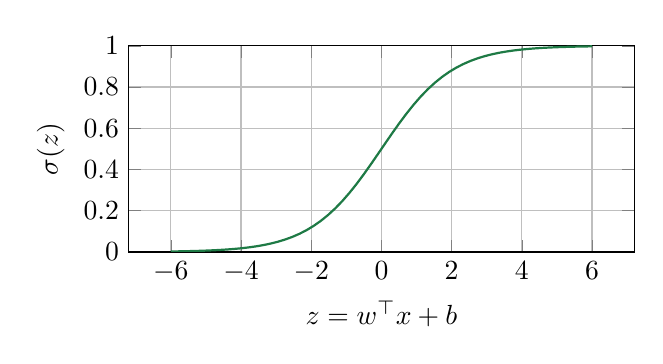
\begin{tikzpicture}\begin{axis}[width=8cm,height=4.2cm,xlabel={$z=w^\top x+b$},ylabel={$\sigma(z)$},domain=-6:6,samples=60,ymin=0,ymax=1,grid=major]
\addplot[AccN,thick]{1/(1+exp(-x))};\end{axis}\end{tikzpicture}\\*{\small\color{GreyN}Figure 2: the sigmoid maps any score to a probability; $z=0$ gives 0.5.}\end{center}
Since $\sigma(z)\ge0.5\iff z\ge0$, the decision boundary $w^\top x+b=0$ is a hyperplane. For $C$ classes the softmax generalisation uses one weight vector per class: $P(y=c\mid x)=e^{w_c^\top x}/\sum_ke^{w_k^\top x}$.

\begin{derivation}{the cross-entropy loss and its gradient}
For labels $y_i\in\{0,1\}$ and predictions $\hat p_i=\sigma(w^\top x_i+b)$, the likelihood is $\prod_i\hat p_i^{y_i}(1-\hat p_i)^{1-y_i}$. Maximising its logarithm is equivalent to minimising the cross-entropy
\[\mathcal L(w)=-\sum_i\big[y_i\log\hat p_i+(1-y_i)\log(1-\hat p_i)\big].\]
Using $\sigma'(z)=\sigma(z)(1-\sigma(z))$, the gradient simplifies to
\[\nabla_w\mathcal L=\sum_i(\hat p_i-y_i)\,x_i,\]
the prediction error times the input. There is no closed-form solution, but the loss is convex, so gradient descent reaches the global optimum.
\end{derivation}

\subsection{Interpreting the weights}
$\log\frac{P(y=1|x)}{1-P(y=1|x)}=w^\top x+b$: each weight is the change in the log-odds per unit change in a feature, and $e^{w_j}$ is the \textbf{odds ratio}. For the adversary-bomber class, the EW-jamming weight is $w_9=4.07$, so jamming multiplies the odds of ``bomber'' by $e^{4.07}=58.5$ --- the strongest predictor, followed by PRF ($+3.12$) and Doppler ($+2.88$).

\subsection{Results and limitations}
One-versus-rest logistic regression achieves 89.7\% test accuracy (macro-F1 0.897) with 0.8 s training and 0.09 ms inference, but adversary-bomber recall is only 87.4\%: one bomber in eight is missed. Its limitations are structural:
\begin{itemize}
\item \textbf{XOR-type classes.} Low, slow UAVs and civilian helicopters occupy interleaved regions that no single hyperplane can separate.
\item \textbf{Interactions.} Danger arises from high speed \emph{and} high PRF together; an additive model $w_1x_1+w_2x_2$ cannot represent ``and'' unless a product feature $x_1x_2$ is added.
\item \textbf{Non-monotonic effects.} Very high speed suggests a threat, except for supersonic civilian jets; a single weight per feature cannot express this.
\end{itemize}

\section{k-Nearest Neighbours}
\subsection{Algorithm}
kNN stores the training set. To classify a query $x_q$: compute the distance $d(x_q,x_i)=\|x_q-x_i\|_2$ to every training point, take the $k$ nearest (the set $N_k(x_q)$), and predict the majority class $\hat y=\arg\max_c\sum_{x_i\in N_k}\mathbf 1[y_i=c]$, optionally weighting votes by $1/d$. There is no training phase; the boundary is a patchwork of Voronoi cells.

\subsection{Choosing $k$}
$k=1$ gives 100\% training accuracy and high variance; $k=N$ predicts the majority class everywhere (high bias). On the IADS data, validation accuracy rose from 78.3\% ($k=1$) to a peak of 90.2\% at $k=21$ (test 89.8\%) and fell to 79.3\% at $k=101$. The heuristic $k\approx\sqrt N\approx76$ is only a starting point.

\subsection{Cost and dimensionality}
Each query costs $O(Nd)$: $5{,}780\times11\approx63{,}600$ operations and 12.2 ms here, borderline for real-time air defence; k-d trees or ball trees reduce the average cost to $O(\log N)$. In high dimensions all points become nearly equidistant (the \textbf{curse of dimensionality}), so distances lose meaning beyond roughly 20 informative dimensions. kNN's strengths are instant updating with new signatures and native multi-class support.

\section{Decision Trees}
\subsection{Impurity and splitting}
A tree recursively splits the data on one feature at a time, choosing at each node the feature $j$ and threshold $t$ that most reduce impurity:
\[G=1-\sum_cp_c^2\ \ \text{(Gini)},\qquad H=-\sum_cp_c\log_2p_c\ \ \text{(entropy)},\]
\[\Delta=I(\text{parent})-\tfrac{n_L}{n}I(L)-\tfrac{n_R}{n}I(R).\]
Splitting stops at a maximum depth, a minimum node size, or a pure node.

\begin{example}{the IADS root split}
At the root, all five classes have $p_c=0.2$, so $G=1-5(0.2^2)=0.80$. Splitting on EW jamming ($x_9\le0.5$) sends 3,120 tracks left (FF 0.32, AB 0.04, CM 0.28, UV 0.24, CI 0.12; $G_L=0.748$) and 2,660 right (FF 0.06, AB 0.48, CM 0.18, UV 0.14, CI 0.14; $G_R=0.694$). Weighted impurity $=\tfrac{3120}{5780}(0.748)+\tfrac{2660}{5780}(0.694)=0.404+0.319=0.723$. The reduction $0.800-0.723=0.077$ is the largest available, so EW jamming becomes the root.
\end{example}

\subsection{Depth, pruning and interpretability}
Test accuracy peaked at depth 10 (91.8\%, 317 nodes); at depth 20 training accuracy reached 99.8\% while test accuracy fell to 88.7\% (2,103 nodes). \textbf{Cost-complexity pruning} minimises $R(T)+\alpha|T|$ (error plus a penalty per leaf); with $\alpha=0.002$ the tree shrank from 317 to 89 nodes while test accuracy \emph{rose} to 92.4\%. Each prediction is an auditable chain of IF--THEN conditions, e.g.\ \texttt{IF jamming AND PRF > 2400 AND speed > 650 THEN AB (91.4\%)} --- valuable for rules-of-engagement compliance. \textbf{Feature importance} sums the impurity reductions contributed by each feature: EW jamming 0.241, PRF 0.187, speed 0.142.

\section{Random Forests}
\subsection{Bagging with feature sub-sampling}
A random forest trains $B$ deep trees, each on a bootstrap sample (drawn with replacement; about 63.2\% of distinct examples appear), and at each split considers only $m\approx\sqrt d$ randomly chosen features ($m=3$ here). Prediction is by majority vote.
\begin{derivation}{why averaging decorrelated trees reduces variance}
If each tree's prediction has variance $\sigma^2$ and pairwise correlation $\rho$, the variance of the average of $B$ trees is
\[\text{Var}=\rho\sigma^2+\frac{1-\rho}{B}\sigma^2.\]
As $B\to\infty$ the second term vanishes but the first remains, so reducing the correlation $\rho$ between trees --- which is what random feature selection does --- is essential. Bias is unchanged by averaging.
\end{derivation}
The roughly 36.8\% of examples left out of each bootstrap sample (``out-of-bag'') provide a free validation estimate.

\subsection{Results}
With $B=500$, $m=3$, unlimited depth and minimum leaf size 2: test accuracy 97.5\%, macro-F1 0.975, out-of-bag error 2.7\% (matching the test error), training 12.4 s, inference 2.8 ms. Per-class F1 ranges from 0.967 (AB) to 0.987 (CI). Permutation importance (the drop in accuracy when a feature is shuffled) again ranks EW jamming (0.228), PRF (0.194) and speed (0.147) highest.

\section{Gradient Boosting and XGBoost}
Boosting builds trees \emph{sequentially}; each new tree fits the residual errors of the ensemble so far:
\[r_{im}=y_i-F_{m-1}(x_i),\qquad F_m(x)=F_{m-1}(x)+\eta\,T_m(x),\]
with a small learning rate $\eta$. Bagging reduces variance using independent trees; boosting reduces bias (and some variance) using dependent ones. XGBoost adds a second-order (Newton) approximation of the loss, regularisation of tree complexity $\Omega(T)=\gamma|T|+\tfrac12\lambda\|w\|^2$, row and column sub-sampling, and fast histogram-based split finding. With 400 trees, $\eta=0.05$ and depth 5, XGBoost reached 96.4\% accuracy and the best adversary-bomber recall (96.8\%), with the fastest inference (0.7 ms) and a compact model suited to embedded hardware.

\section{Support Vector Machines}
\subsection{The maximum-margin hyperplane}
For linearly separable classes $y_i\in\{-1,+1\}$, infinitely many hyperplanes separate the data. The SVM chooses the one with the largest \textbf{margin}, the distance to the nearest points.
\begin{derivation}{margin and the primal problem}
The distance from $x_i$ to the hyperplane $w^\top x+b=0$ is $|w^\top x_i+b|/\|w\|$. Rescale $w,b$ so that the closest points satisfy $y_i(w^\top x_i+b)=1$; the margin is then $2/\|w\|$. Maximising it is equivalent to
\[\min_{w,b}\tfrac12\|w\|^2\quad\text{subject to}\quad y_i(w^\top x_i+b)\ge1\ \ \forall i,\]
a convex quadratic programme with a unique solution. Introducing Lagrange multipliers $\alpha_i\ge0$ gives the dual
\[\max_\alpha\sum_i\alpha_i-\tfrac12\sum_{i,j}\alpha_i\alpha_jy_iy_j\,x_i^\top x_j,\qquad w^*=\sum_i\alpha_iy_ix_i.\]
Only the \textbf{support vectors} (points on the margin) have $\alpha_i>0$, and the data enter only through inner products $x_i^\top x_j$.
\end{derivation}
\begin{center}\begin{tikzpicture}[x=0.9cm,y=0.9cm]
\draw[GreyN](0,0)rectangle(5,4);\foreach \x/\y in {0.6/3.4,1.2/2.9,0.7/2.3,1.7/3.5,1.9/2.6}{\fill[BluN](\x,\y)circle(0.08);}\foreach \x/\y in {3.3/0.5,4.1/1.1,3.8/0.4,4.4/1.7,3.0/1.3}{\fill[RedN](\x,\y)circle(0.08);}
\draw[AccN,thick](0.7,0.2)--(4.4,3.8);\draw[AccN,dashed](0.2,0.5)--(3.9,4.1);\draw[AccN,dashed](1.2,-0.1)--(4.9,3.5);
\draw[GrnN,thick](1.9,2.6)circle(0.2);\draw[GrnN,thick](3.0,1.3)circle(0.2);\node[font=\scriptsize,anchor=west]at(5.1,2){support vectors circled; margin $=2/\|w\|$};
\end{tikzpicture}\\*{\small\color{GreyN}Figure 3: the maximum-margin hyperplane (solid) and its margin (dashed).}\end{center}
A wide margin makes the classifier robust to sensor noise and to small variations in an adversary's signature.

\subsection{Soft margin}
When classes overlap, slack variables $\xi_i\ge0$ allow violations:
\[\min\tfrac12\|w\|^2+C\sum_i\xi_i\quad\text{s.t.}\quad y_i(w^\top x_i+b)\ge1-\xi_i.\]
$\xi_i=0$: correct and outside the margin; $0<\xi_i<1$: inside the margin but correct; $\xi_i>1$: misclassified. Small $C$ tolerates violations (wide margin, risk of underfitting); large $C$ penalises them (narrow margin, risk of overfitting). On the IADS data, validation accuracy rose from 74.2\% ($C=0.01$) to 95.4\% ($C=100$) and fell slightly beyond. Asymmetric costs can be encoded with class-specific $C$, e.g.\ $C_{AB}=5C$.

\subsection{The kernel trick}
Because the dual uses only inner products, we can replace $x_i^\top x_j$ with a \textbf{kernel} $K(x_i,x_j)=\phi(x_i)^\top\phi(x_j)$, an inner product in a higher-dimensional feature space, without ever computing $\phi$.
\begin{example}{a one-dimensional illustration}
Points with $|x|$ small belong to class A and points with $|x|$ large to class B: no single threshold on the line separates them. Mapping $\phi(x)=(x,x^2)$ lifts them onto a parabola where the horizontal line $x^2=c$ separates the classes. The polynomial kernel $K(x,x')=(xx'+1)^2$ performs such a mapping implicitly; for $d=11$ features the degree-2 kernel corresponds to a 78-dimensional space.
\end{example}
The \textbf{RBF kernel} $K(x,x')=\exp(-\gamma\|x-x'\|^2)$ corresponds to an infinite-dimensional space; small $\gamma$ gives smooth boundaries, large $\gamma$ very local ones. A grid search on the IADS data found the best $\gamma=0.08$, $C=100$ (95.4\% validation); the final model reached 96.7\% test accuracy with 1,247 support vectors (21.6\% of the training set), 38.4 s training and 4.1 ms inference. Kernels must be symmetric and positive semi-definite (Mercer's condition). Specialised kernels exist for spectra, time series (dynamic time warping) and symbol strings.

\section{Naive Bayes}
Bayes' theorem with the ``naive'' assumption that features are conditionally independent given the class gives
\[P(y=c\mid x)\propto P(y=c)\prod_{j=1}^dP(x_j\mid y=c),\]
with Gaussian likelihoods $P(x_j\mid c)=\mathcal N(x_j;\mu_{cj},\sigma_{cj}^2)$ for continuous features. Prediction uses logarithms to avoid underflow: $\hat y=\arg\max_c[\log P(c)+\sum_j\log P(x_j|c)]$. Training only estimates class means and variances, so it is extremely fast.
\begin{example}{classifying by PRF}
FF tracks have PRF $\mu=1040$, $\sigma=185$ Hz; AB tracks $\mu=2280$, $\sigma=310$ Hz. A new track has PRF 1,950 Hz. For FF, $z=(1950-1040)/185=4.92$ --- extremely unlikely; for AB, $z=(1950-2280)/310=-1.06$ --- plausible. The likelihood ratio strongly favours AB.
\end{example}
On the IADS data Naive Bayes reached only 83.1\% accuracy and 79.3\% AB recall --- the weakest model --- because PRF and speed are strongly correlated for bombers, violating the independence assumption. It remains useful for text, streaming data, small samples and fast baselines.

\section{Multi-class Strategies, Calibration and Rejection}
\textbf{One-vs-rest} trains $C$ binary classifiers (each class against all others); \textbf{one-vs-one} trains $C(C-1)/2$ (10 for five classes) and takes a majority vote; trees, forests, Naive Bayes and softmax regression are natively multi-class. For logistic regression the three approaches gave 89.7\%, 90.1\% and 89.9\%.

Raw classifier scores are not probabilities. \textbf{Calibration} maps scores to reliable probabilities: Platt scaling fits a sigmoid to SVM scores; isotonic regression fits a monotone step function. A commander needs ``80\% confident this is a bomber'', not just a label. A \textbf{reject option} refers low-confidence cases to a human: with threshold 0.6, 4.2\% of tracks were referred to analysts (who were 98.7\% accurate on them), raising combined system accuracy to 99.1\%.

\section{Class Imbalance}
On the real IADS stream (78.4\% civilian, 14.2\% friendly, 4.8\% UAV, 1.8\% missile, 0.8\% bomber), a model trained naively labels almost everything civilian: accuracy 92.6\%, but bomber recall only 12.3\%. Loss minimisation simply learns the class frequencies.
\begin{itemize}
\item \textbf{SMOTE oversampling:} create synthetic minority examples $x_{\text{new}}=x_i+\lambda(x_j-x_i)$, $\lambda\sim U(0,1)$, between a minority example and one of its minority neighbours. Bomber recall rose from 12\% to 89\%.
\item \textbf{Undersampling} the majority class: fast but discards information.
\item \textbf{Class weights:} $w_c=N/(C\cdot N_c)$; with 43 bombers among 5,780 training tracks, $w_{AB}=5780/(5\times43)=26.9$.
\item \textbf{Threshold shifting:} classify as bomber when $P(\text{AB}|x)>0.15$ instead of 0.5, accepting more false alarms when a miss is far costlier.
\end{itemize}
\begin{pitfall}{SMOTE before splitting}
Generating synthetic examples before the train/test split leaks information: synthetic test points are interpolations of training points. Always split first, then oversample the training fold only.
\end{pitfall}

\section{Comparing the Classifiers}
\begin{center}\small\renewcommand{\arraystretch}{1.2}
\begin{tabular}{lcccccc}\toprule Algorithm & Train & Test & F1 & AB recall & Train (s) & Infer (ms)\\\midrule
Logistic regression & 95.4\% & 89.7\% & 0.897 & 87.4\% & 0.8 & 0.09\\ kNN ($k=21$) & 91.8\% & 89.8\% & 0.894 & 88.2\% & --- & 12.2\\ Decision tree ($d=10$) & 95.7\% & 91.8\% & 0.915 & 90.4\% & 0.5 & 0.15\\ \textbf{Random forest} & 99.2\% & \textbf{97.5\%} & \textbf{0.975} & 96.1\% & 12.4 & 2.8\\ XGBoost & 98.7\% & 96.4\% & 0.963 & \textbf{96.8\%} & 18.6 & \textbf{0.7}\\ SVM (RBF) & 97.8\% & 96.7\% & 0.967 & 95.2\% & 38.4 & 4.1\\ Naive Bayes & 89.1\% & 83.1\% & 0.826 & 79.3\% & 0.03 & 0.02\\\bottomrule\end{tabular}\end{center}
Random forest wins on accuracy; XGBoost on speed and bomber recall; the decision tree on interpretability. Naive Bayes misses one bomber in five and should not be used here. These are results on one balanced test set of 1,275 tracks without confidence intervals: differences of a fraction of a point (e.g.\ SVM 96.7\% vs XGBoost 96.4\%) are not meaningful.

\section{Evaluation Beyond Accuracy}
\subsection{ROC curves and AUC}
Sweeping the decision threshold traces the \textbf{ROC curve} of true-positive rate $TP/(TP+FN)$ against false-positive rate $FP/(FP+TN)$. The area under it (AUC) is the probability that a randomly chosen positive is scored above a randomly chosen negative: 0.5 is random, 1.0 perfect. For the AB class (one-vs-rest): random forest 0.998, SVM 0.996, logistic regression 0.963, decision tree 0.940, Naive Bayes 0.912. At a 5\% false-alarm rate, random forest detects 97.8\% of bombers and logistic regression 88.3\%.

\begin{center}\begin{tikzpicture}\begin{axis}[width=8.5cm,height=6cm,xlabel={false-positive rate},ylabel={true-positive rate},xmin=0,xmax=1,ymin=0,ymax=1,domain=0:1,samples=80,legend pos=south east,grid=major]
\addplot[GrnN,thick]{1-(1-x)^499};\addlegendentry{RF (0.998)}\addplot[BluN,thick]{1-(1-x)^26};\addlegendentry{LR (0.963)}\addplot[RedN,thick]{1-(1-x)^10.4};\addlegendentry{NB (0.912)}\addplot[GreyN,dashed]{x};\addlegendentry{random}
\end{axis}\end{tikzpicture}\\*{\small\color{GreyN}Figure 4: schematic ROC curves drawn to match the reported AUCs (shapes illustrative).}\end{center}
\subsection{Precision--recall under imbalance}
When positives are rare, FPR stays small even when false alarms vastly outnumber true detections (the base-rate effect of Lecture~1). The precision--recall curve and its summary, \textbf{average precision} $AP=\sum_k(R_k-R_{k-1})P_k$, are more informative: on the real stream, AP for bombers was 0.887 (RF), 0.642 (LR) and 0.441 (NB). The $F_\beta$ score weights recall $\beta$ times as much as precision:
\[F_\beta=(1+\beta^2)\frac{PR}{\beta^2P+R}.\]
$\beta=2$ suits the IADS bomber class, where a miss is much costlier than a false alarm: $F_2=0.974$ (RF) vs 0.894 (LR).

\section{Deeper Dive I: Data Preparation in Practice}
\subsection{Encoding and scaling}
Classifiers need numeric inputs on comparable scales. \textbf{Standardisation} $\tilde x_j=(x_j-\mu_j)/\sigma_j$ gives each feature mean 0 and variance 1; \textbf{min--max scaling} maps to $[0,1]$ but is sensitive to outliers. Categorical features such as polarisation (horizontal, vertical, circular) are \textbf{one-hot encoded} as three binary columns; encoding them as 1, 2, 3 would wrongly imply an order and equal spacing.
\begin{pitfall}{fitting the scaler on all data}
The scaling parameters $\mu_j,\sigma_j$ must be computed from the training fold only and then applied to validation and test data. Computing them on the whole dataset leaks information about the test distribution into training --- a small but real form of data leakage.
\end{pitfall}

\subsection{Stratified splitting}
When classes are imbalanced, a random split may leave the rare class almost absent from a fold. \textbf{Stratified} splitting preserves class proportions in every fold. With 43 bombers in 5,780 training tracks, a random 5-fold split could put as few as 4--5 bombers in a validation fold, making recall estimates extremely noisy; stratification guarantees about 8--9 per fold.

\subsection{Leakage examples from defence data}
\begin{itemize}
\item \textbf{Temporal leakage:} random splits of a track stream place radar returns from the same aircraft in both training and test sets; the model recognises the individual track, not the class. Split by track, sortie or day.
\item \textbf{Label leakage:} a ``track status'' field populated by the operator \emph{after} classification encodes the answer.
\item \textbf{Duplicate leakage:} identical simulator scenarios replayed with different random seeds appear in both sets.
\end{itemize}

\section{Deeper Dive II: Training Logistic Regression}
\subsection{One step of gradient descent by hand}
\begin{example}{a single update}
One training example has features $x=(1,\,2)$ (bias term included as the first entry), label $y=1$, current weights $w=(0,\,0.5)$, learning rate $\alpha=0.1$.
\begin{enumerate}
\item Score: $z=w^\top x=0+0.5\times2=1.0$; prediction $\hat p=\sigma(1)=0.731$.
\item Loss: $-\log0.731=0.313$.
\item Gradient: $(\hat p-y)x=(-0.269)(1,2)=(-0.269,-0.538)$.
\item Update: $w\leftarrow w-\alpha\nabla=(0.0269,\;0.5538)$.
\end{enumerate}
The new score is $0.0269+1.1076=1.1345$, $\hat p=0.757$: the prediction moved toward the label. Repeating over all examples (an epoch) and many epochs converges because the loss is convex.
\end{example}

\subsection{Regularised logistic regression}
Adding $\lambda\|w\|^2$ (L2) or $\lambda\|w\|_1$ (L1) to the cross-entropy prevents weights from growing without bound when classes are perfectly separable, and L1 selects features. In scikit-learn the parameter $C=1/\lambda$: small $C$ means strong regularisation.

\subsection{Softmax worked example}
\begin{example}{three-class probabilities}
For a track, class scores are $z_{\text{FF}}=2.0$, $z_{\text{AB}}=1.0$, $z_{\text{CI}}=0.1$. Exponentials: 7.389, 2.718, 1.105; sum 11.212. Probabilities: FF 0.659, AB 0.242, CI 0.099. Adding a constant to all scores leaves the probabilities unchanged, which is why implementations subtract the largest score before exponentiating (numerical stability).
\end{example}

\begin{center}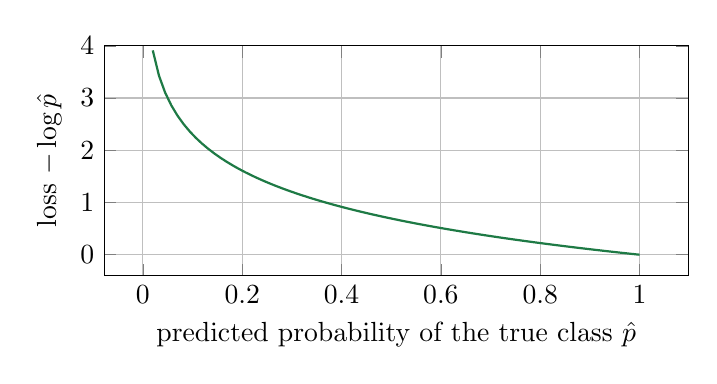
\begin{tikzpicture}\begin{axis}[width=9cm,height=4.5cm,xlabel={predicted probability of the true class $\hat p$},ylabel={loss $-\log\hat p$},domain=0.02:1,samples=80,grid=major,ymax=4]
\addplot[AccN,thick]{-ln(x)};\end{axis}\end{tikzpicture}\\*{\small\color{GreyN}Figure 5: cross-entropy punishes confident mistakes severely ($-\log0.02\approx3.9$).}\end{center}

\section{Deeper Dive III: Distances, Trees and Ensembles}
\subsection{kNN by hand}
\begin{example}{classifying one track with $k=3$}
Standardised training tracks (PRF, speed) and labels: A $(0.2,0.1)$ FF; B $(0.5,0.4)$ FF; C $(1.8,1.6)$ AB; D $(2.1,1.9)$ AB; E $(1.2,1.0)$ AB. Query $q=(1.0,0.9)$. Euclidean distances: A 1.13, B 0.71, C 1.06, D 1.49, E 0.22. The three nearest are E (AB), B (FF), C (AB): majority AB. With $k=1$ the answer is also AB; with $k=5$ it is AB 3--2. Distance-weighted voting ($1/d$): AB $=4.47+0.94+0.67=6.08$, FF $=1.41+0.88=2.29$ for $k=5$.
\end{example}
Other metrics: Manhattan $\sum|x_j-x'_j|$ (robust to single large differences), Mahalanobis (accounts for correlation), cosine (for direction rather than magnitude, e.g.\ spectra).

\subsection{Entropy and information gain}
\begin{example}{entropy for the root split}
Parent: five equal classes, $H=\log_25=2.32$ bits. Left child (0.32, 0.04, 0.28, 0.24, 0.12): $H=-\sum p\log_2p=0.526+0.186+0.514+0.494+0.367=2.09$ bits. Right child (0.06, 0.48, 0.18, 0.14, 0.14): $H=0.244+0.508+0.445+0.397+0.397=1.99$ bits. Weighted child entropy $=0.54(2.09)+0.46(1.99)=2.04$; information gain $=0.28$ bits. Gini and entropy almost always choose the same split; Gini is slightly cheaper to compute.
\end{example}

\begin{center}\begin{tikzpicture}[level distance=1.3cm,sibling distance=3.6cm,every node/.style={nd,font=\scriptsize}]
\node{EW jamming?}
 child{node{Speed $<250$?} child{node[fill=GrnN!15]{Civilian 93.7\%}} child{node{Pulse width $<0.8$?} child{node[fill=GrnN!15]{CM 88.2\%}} child{node{\ldots}}}}
 child{node{PRF $>2400$?} child{node{Speed $>650$?} child{node[fill=RedN!15]{AB 91.4\%}} child{node{\ldots}}} child{node{\ldots}}};
\end{tikzpicture}\\*{\small\color{GreyN}Figure 6: top of the pruned IADS tree --- every prediction is an auditable rule.}\end{center}

\subsection{The bootstrap and out-of-bag fraction}
\begin{derivation}{why about 36.8\% of examples are out of bag}
Drawing $N$ times with replacement, a given example is missed on each draw with probability $1-1/N$, so it is absent from the whole bootstrap sample with probability $(1-1/N)^N\to e^{-1}\approx0.368$ as $N\to\infty$. Hence about 63.2\% of distinct examples are in each sample and 36.8\% are out of bag.
\end{derivation}

\subsection{Feature-importance pitfalls}
Impurity-based importance favours features with many possible split points (continuous or high-cardinality features) and splits credit unpredictably among correlated features. \textbf{Permutation importance} --- the drop in validation accuracy when one feature's values are shuffled --- is more reliable; \textbf{SHAP values} decompose each individual prediction into feature contributions and are preferred for explaining specific decisions to commanders.

\subsection{AdaBoost: the original boosting algorithm}
AdaBoost (Freund \& Schapire, 1997) re-weights training examples. Starting with equal weights, at round $m$ it trains a weak learner, computes its weighted error $\epsilon_m$, gives it a vote $\alpha_m=\tfrac12\ln\frac{1-\epsilon_m}{\epsilon_m}$, and multiplies the weights of misclassified examples by $e^{\alpha_m}$ (correct ones by $e^{-\alpha_m}$) before renormalising. A learner with $\epsilon=0.2$ gets $\alpha=0.69$; one with $\epsilon=0.45$ gets only $0.10$. Gradient boosting generalises this idea to any differentiable loss.

\section{Deeper Dive IV: Costs, Calibration and Comparing Models}
\subsection{The cost-optimal threshold}
\begin{derivation}{when to declare a threat}
Let $p=P(\text{AB}\mid x)$ be calibrated, $C_{FN}$ the cost of missing a bomber and $C_{FP}$ the cost of a false alarm. Declaring ``bomber'' has expected cost $(1-p)C_{FP}$; declaring ``not bomber'' has expected cost $pC_{FN}$. Declare a threat when $pC_{FN}>(1-p)C_{FP}$, i.e.
\[p>\frac{C_{FP}}{C_{FP}+C_{FN}}.\]
If a miss is 20 times as costly as a false alarm, the threshold is $1/21\approx0.048$, not 0.5.
\end{derivation}
This only works if probabilities are calibrated --- which is why calibration matters operationally.

\subsection{Measuring calibration}
A \textbf{reliability diagram} plots observed frequency against predicted probability in bins; a calibrated model lies on the diagonal. The \textbf{Brier score} $\frac1N\sum(p_i-y_i)^2$ combines calibration and discrimination (lower is better). Boosted trees and SVM scores are often poorly calibrated and benefit from Platt or isotonic recalibration on held-out data.

\begin{center}\begin{tikzpicture}\begin{axis}[width=7cm,height=5.5cm,xlabel={predicted probability},ylabel={observed frequency},xmin=0,xmax=1,ymin=0,ymax=1,grid=major,legend pos=north west]
\addplot[GreyN,dashed,domain=0:1]{x};\addlegendentry{perfect}
\addplot[RedN,thick,mark=*]coordinates{(0.05,0.12)(0.25,0.33)(0.45,0.47)(0.65,0.60)(0.85,0.71)(0.95,0.78)};\addlegendentry{uncalibrated}
\addplot[GrnN,thick,mark=square*]coordinates{(0.05,0.06)(0.25,0.26)(0.45,0.44)(0.65,0.66)(0.85,0.83)(0.95,0.93)};\addlegendentry{after isotonic}
\end{axis}\end{tikzpicture}\\*{\small\color{GreyN}Figure 7: an illustrative reliability diagram.}\end{center}

\subsection{Is one classifier really better? Confidence intervals and McNemar's test}
A test accuracy $\hat a$ on $n$ examples has standard error $\sqrt{\hat a(1-\hat a)/n}$. For RF, $\hat a=0.975$, $n=1{,}275$: SE $=0.0044$, so the 95\% interval is about $97.5\%\pm0.9\%$. SVM's 96.7\% and XGBoost's 96.4\% lie close to or inside that range, so the ranking among the top three is uncertain. Because both models are scored on the \emph{same} test examples, the right test is \textbf{McNemar's}: let $b$ be the number of examples RF gets right and SVM wrong, and $c$ the reverse; under $H_0$ (equal accuracy) $\chi^2=(b-c)^2/(b+c)$ has one degree of freedom.
\begin{example}{McNemar}
If $b=25$ and $c=15$, $\chi^2=100/40=2.5$, $p=0.11$: no significant difference despite RF's higher accuracy. Lecture~1's warning applies: small differences between strong models are often noise.
\end{example}

\clearpage
\part*{Part C --- Further Theory, Methods and Applications}
\addcontentsline{toc}{part}{Part C --- Further Theory, Methods and Applications}

\section{Why Learning Generalises: Capacity and Sample Size}
A classifier's training accuracy is an optimistic estimate of its accuracy on new data. How optimistic depends on two things: how flexible the model family is, and how much data it was fitted to. Statistical learning theory makes this precise.

\subsection{Shattering and the VC dimension}
A model family \textbf{shatters} a set of points if, for every one of the $2^n$ ways of labelling those points, some member of the family classifies them all correctly. The \textbf{Vapnik--Chervonenkis (VC) dimension} is the largest number of points the family can shatter.
\begin{example}{lines in the plane}
Three points not on a line can be labelled in $2^3=8$ ways, and for every labelling a straight line separates the positives from the negatives: lines shatter three points. No four points can be shattered --- the XOR arrangement (opposite corners of a square sharing a label) defeats every line. So linear classifiers in two dimensions have VC dimension 3; in $d$ dimensions, $d+1$.
\end{example}
A classic bound states that, with probability at least $1-\delta$, the true error $E$ of a classifier from a family of VC dimension $h$, trained on $N$ examples with training error $E_{\text{train}}$, satisfies
\[E\le E_{\text{train}}+\sqrt{\frac{h\big(\ln(2N/h)+1\big)+\ln(4/\delta)}{N}}.\]
The numbers it produces are loose, but the shape is the lesson: the gap between training and true error grows with capacity $h$ and shrinks roughly as $1/\sqrt N$. A family that can fit anything (a 1-NN classifier, an unpruned tree) has an uninformative bound, which is why such models must be judged on held-out data.

\subsection{Bias and variance of $k$-NN}
For $k$-NN regression with noise variance $\sigma^2$, the variance of a prediction is about $\sigma^2/k$: averaging more neighbours reduces noise. But larger $k$ reaches further away for neighbours, whose true values differ from the query's, so bias grows. With $N$ points and $k$ neighbours the model has roughly $N/k$ \emph{effective parameters}. On the IADS data, $k=1$ gave 78.3\% validation accuracy and $k=21$ gave 90.2\%: the noise-averaging gain outweighed the bias at that scale.

\section{Logistic Regression as Maximum Likelihood}
\subsection{Deriving the loss}
Model the label as a Bernoulli variable with $P(y=1\mid x)=p(x)=\sigma(w^\top x+b)$. The likelihood of independent training labels is $\prod_ip_i^{y_i}(1-p_i)^{1-y_i}$; its negative logarithm is
\[-\ell(w,b)=-\sum_i\big[y_i\ln p_i+(1-y_i)\ln(1-p_i)\big],\]
which is exactly the cross-entropy loss. Minimising cross-entropy is therefore \textbf{maximum-likelihood estimation}. The loss is convex in $(w,b)$, so gradient descent cannot get stuck in a poor local minimum.
\subsection{Newton's method (IRLS)}
Because the loss is smooth and convex, Newton's method converges in a handful of iterations: $w\leftarrow w-H^{-1}\nabla\ell$, with gradient $X^\top(p-y)$ and Hessian $H=X^\top SX$, where $S=\text{diag}\big(p_i(1-p_i)\big)$. Each step is a weighted least-squares problem, hence the name \emph{iteratively re-weighted least squares}. Statistical packages use it, and $H^{-1}$ at the optimum gives standard errors for the weights.
\subsection{Geometry and a failure mode}
The decision boundary $p=0.5$ is the hyperplane $w^\top x+b=0$, and $|w^\top x+b|/\|w\|$ is a point's distance from it: the further away, the more confident the prediction. If the classes are \textbf{perfectly separable}, the likelihood keeps increasing as $\|w\|\to\infty$; the weights diverge and the probabilities become 0 and 1. Small defence datasets with many features are often separable by chance; L2 regularisation keeps the weights finite and the probabilities honest.
\subsection{More than two classes}
Multinomial (softmax) regression gives each class $k$ a weight vector $w_k$ and sets $P(y=k\mid x)=e^{w_k^\top x}/\sum_je^{w_j^\top x}$. The gradient for class $k$ is $(p_k-\mathbf 1[y=k])\,x$ --- the same simple form as the binary case.

\section{From the Perceptron to the Support Vector Machine}
\subsection{The perceptron algorithm}
With labels $y\in\{-1,+1\}$, the perceptron predicts $\text{sign}(w^\top x+b)$ and, whenever an example is misclassified ($y(w^\top x+b)\le0$), updates $w\leftarrow w+yx$, $b\leftarrow b+y$.
\begin{example}{perceptron by hand}
Training points: $(1,1)$ and $(2,-1)$ are hostile ($+1$); $(-1,1)$ and $(0,-2)$ are friendly ($-1$). Start with $w=(0,0)$, $b=0$.\\
Point $(1,1)$: score 0, misclassified $\Rightarrow w=(1,1)$, $b=1$. Point $(2,-1)$: score $2$, correct. Point $(-1,1)$: score $1$ but label $-1$ $\Rightarrow w=(2,0)$, $b=0$. Point $(0,-2)$: score 0, misclassified $\Rightarrow w=(2,2)$, $b=-1$.\\
Second pass: margins $y(w^\top x+b)$ are $3,1,1,5$ --- all positive. Converged: $2x_1+2x_2-1=0$ separates the classes.
\end{example}
\textbf{Novikoff's theorem:} if the data are separable with margin $\gamma$ and all points lie within radius $R$, the perceptron makes at most $(R/\gamma)^2$ mistakes. It finds \emph{a} separating line, but which one depends on the order of the data. The SVM asks for the \emph{best} one.

\subsection{The SVM optimisation problem and its dual}
The hard-margin SVM solves $\min\frac12\|w\|^2$ subject to $y_i(w^\top x_i+b)\ge1$. Introducing a Lagrange multiplier $\alpha_i\ge0$ for each constraint gives the Lagrangian
\[L=\tfrac12\|w\|^2-\textstyle\sum_i\alpha_i\big[y_i(w^\top x_i+b)-1\big].\]
Setting derivatives to zero yields $w=\sum_i\alpha_iy_ix_i$ and $\sum_i\alpha_iy_i=0$. Substituting back gives the \textbf{dual problem}:
\[\max_\alpha\;\sum_i\alpha_i-\tfrac12\sum_i\sum_j\alpha_i\alpha_jy_iy_j\,x_i^\top x_j\quad\text{s.t. }\alpha_i\ge0,\;\textstyle\sum_i\alpha_iy_i=0.\]
The \textbf{Karush--Kuhn--Tucker conditions} require $\alpha_i[y_i(w^\top x_i+b)-1]=0$: either $\alpha_i=0$ (the point is beyond the margin and plays no role) or the point lies exactly on the margin. Points with $\alpha_i>0$ are the \textbf{support vectors}; the solution depends on them alone. With the soft margin, the only change is $0\le\alpha_i\le C$.
\begin{example}{an SVM solved by hand}
Hostile tracks at $(3,3)$ and $(3,4)$; a friendly track at $(1,1)$. By symmetry the boundary is perpendicular to the segment from $(1,1)$ to $(3,3)$ and passes through its midpoint $(2,2)$: $w\propto(1,1)$. The margin constraints $w^\top x+b=\pm1$ at $(3,3)$ and $(1,1)$ give $w=(0.5,0.5)$ and $b=-2$. Check $(3,4)$: $0.5(3)+0.5(4)-2=1.5\ge1$, so it is not a support vector ($\alpha=0$). Margin width $2/\|w\|=2/0.707=2.83$, exactly the distance between $(1,1)$ and $(3,3)$. From $w=\sum\alpha_iy_ix_i=\alpha_1(3,3)-\alpha_3(1,1)$ with $\alpha_1=\alpha_3$: $\alpha(2,2)=(0.5,0.5)$, so $\alpha_1=\alpha_3=0.25$. Moving $(3,4)$ anywhere outside the margin would not change the classifier at all.
\end{example}
\begin{center}\begin{tikzpicture}\begin{axis}[width=6cm,height=5.6cm,xmin=0,xmax=5,ymin=0,ymax=5,grid=both,grid style={GreyN!15},xlabel={$x_1$},ylabel={$x_2$},font=\scriptsize]
\addplot[AccN,thick,domain=0:5]{4-x};\addplot[AccN,dashed,domain=0:5]{6-x};\addplot[AccN,dashed,domain=0:5]{2-x};
\addplot[only marks,mark=*,RedN,mark size=2.5pt]coordinates{(3,3)(3,4)};
\addplot[only marks,mark=square*,BluN,mark size=2.5pt]coordinates{(1,1)};
\node[font=\tiny,anchor=west]at(axis cs:3.15,2.9){SV};\node[font=\tiny,anchor=west]at(axis cs:1.15,0.9){SV};
\node[font=\tiny,AccN,rotate=-45]at(axis cs:1.75,2.6){$w^\top x+b=0$};
\end{axis}\end{tikzpicture}\\*{\small\color{GreyN}Figure C1: the hand-solved SVM. Dashed lines are the margins $w^\top x+b=\pm1$; SV marks the support vectors.}\end{center}


\subsection{Kernels}
The dual uses the data only through inner products $x_i^\top x_j$. Replacing them by a \textbf{kernel} $K(x_i,x_j)=\phi(x_i)^\top\phi(x_j)$ trains a linear SVM in the feature space $\phi$ without ever computing $\phi$.
\begin{example}{a kernel is a hidden inner product}
For the polynomial kernel $K(x,z)=(x^\top z+1)^2$ with $x=(1,2)$, $z=(3,1)$: $x^\top z=5$, so $K=36$. The explicit six-dimensional map $\phi(v)=(1,\sqrt2v_1,\sqrt2v_2,v_1^2,v_2^2,\sqrt2v_1v_2)$ gives $\phi(x)=(1,1.414,2.828,1,4,2.828)$ and $\phi(z)=(1,4.243,1.414,9,1,4.243)$, whose inner product is also 36. The kernel did the work of the six-dimensional map with one multiplication and a square. The RBF kernel $K=\exp(-\gamma\|x-z\|^2)$ corresponds to an infinite-dimensional map; with $\gamma=0.5$ these two points give $e^{-0.5\times5}=0.082$.
\end{example}
\textbf{Mercer's condition}: a function is a valid kernel if every kernel matrix it produces is symmetric and positive semi-definite. Sums and products of valid kernels are valid, so domain-specific kernels (for strings, graphs, time series) can be built from simple ones.
\subsection{The SVM as a regularised loss}
The soft-margin SVM is equivalent to minimising $\frac1N\sum_i\max\big(0,1-y_if(x_i)\big)+\lambda\|w\|^2$: hinge loss plus L2 regularisation. Logistic regression replaces the hinge by the logistic loss $\ln(1+e^{-yf})$. The two give similar boundaries; the hinge ignores points that are confidently correct, which is why only support vectors matter, while logistic regression gives calibrated probabilities. SVM scores are not probabilities; Platt scaling fits a sigmoid to them on validation data when probabilities are needed.

\section{Trees and Ensembles in Depth}
\subsection{The CART algorithm}
\begin{algo}{growing a classification tree (CART)}
\begin{enumerate}[leftmargin=1.5em]
\item At a node, for every feature sort the values and consider thresholds midway between consecutive distinct values.
\item For each candidate split compute the weighted impurity of the two children; choose the split with the largest impurity decrease.
\item Recurse on each child until a stopping rule holds (maximum depth, minimum samples per leaf, or no impurity decrease).
\item Label each leaf with its majority class (or class proportions as probabilities).
\end{enumerate}
\end{algo}
The search is greedy: the best split now may not lead to the best tree. Trees handle mixed feature types and need no scaling, but small changes in data can change the top split and therefore the whole tree --- the instability that ensembles exploit.
\subsection{Cost-complexity pruning}
Grow a large tree, then prune it back by minimising $R_\alpha(T)=R(T)+\alpha|T|$, where $R(T)$ is the training error and $|T|$ the number of leaves. For each internal node, compare the subtree below it with collapsing it to a leaf.
\begin{example}{when to prune}
A subtree with 5 leaves has error 0.10; collapsing it to one leaf gives error 0.16. The two are equally good when $0.10+5\alpha=0.16+\alpha$, i.e.\ $\alpha=0.015$. For any complexity penalty above 0.015 per leaf the subtree is pruned. Increasing $\alpha$ prunes progressively, producing a sequence of trees from which cross-validation picks one.
\end{example}
\textbf{Regression trees} use the same procedure with variance (squared error) as the impurity and the leaf mean as the prediction.

\subsection{How much does bagging help?}
If each of $B$ trees has prediction variance $\sigma^2$ and any two trees have correlation $\rho$, the variance of their average is
\[\rho\sigma^2+\frac{1-\rho}{B}\sigma^2.\]
With $\sigma^2=1$ and $\rho=0.3$: one tree 1.0; ten trees 0.37; a hundred trees 0.307 --- and no number of trees gets below $\rho\sigma^2=0.3$. Reducing the correlation to $\rho=0.05$ (by sampling a random subset of features at each split) brings 100 trees down to 0.06. This formula is the whole design rationale of random forests: decorrelate the trees, then average many of them.

\subsection{Gradient boosting and the XGBoost split gain}
Boosting builds an additive model $F_M(x)=\sum_m\eta\,T_m(x)$, each tree fitted to the negative gradient of the loss at the current predictions (for squared error, the residuals). XGBoost uses first and second derivatives of the loss --- $g_i$ and $h_i$ for each example --- and regularises each tree. For a candidate split of a node into left and right sets, the gain is
\[\text{Gain}=\tfrac12\Big[\frac{G_L^2}{H_L+\lambda}+\frac{G_R^2}{H_R+\lambda}-\frac{(G_L+G_R)^2}{H_L+H_R+\lambda}\Big]-\gamma_{\text{split}},\]
with $G$ and $H$ the sums of $g_i$ and $h_i$ in each set, and optimal leaf values $w=-G/(H+\lambda)$.
\begin{example}{one XGBoost split}
Four examples with squared-error gradients $g=(-2,-1,1,3)$ and $h=1$ each; $\lambda=1$, $\gamma_{\text{split}}=0$. Splitting into $\{-2,-1\}$ and $\{1,3\}$: $G_L=-3$, $G_R=4$, $H_L=H_R=2$. Gain $=\frac12[9/3+16/3-1/5]=4.07$. Leaf values: left $+1.0$, right $-1.33$ --- each leaf moves its predictions against its gradient, i.e.\ toward the targets, shrunk by $\lambda$.
\end{example}

\subsection{Stacking and voting}
\textbf{Hard voting} takes the majority class of several models; \textbf{soft voting} averages their probabilities. \textbf{Stacking} trains a second-level model on the out-of-fold predictions of the first-level models, learning when to trust which. Ensembles of diverse models (a forest, an SVM and a neural network) often beat each member, but the gain shrinks when members make the same errors.

\section{Probabilistic Classifiers in Depth}
\subsection{Gaussian Naive Bayes worked fully}
\begin{example}{bomber or fighter from speed and radar cross-section}
Training data give: bombers (prior 0.3) speed $\sim\mathcal N(850,100^2)$ km/h, RCS $\sim\mathcal N(20,8^2)$ m$^2$; fighters (prior 0.7) speed $\sim\mathcal N(1100,250^2)$, RCS $\sim\mathcal N(5,3^2)$. A track flies at 950 km/h with RCS 12 m$^2$.\\
Likelihoods: bomber speed density $2.42\times10^{-3}$, RCS $3.03\times10^{-2}$; fighter speed $1.33\times10^{-3}$, RCS $8.74\times10^{-3}$.\\
Unnormalised posteriors: bomber $0.3\times2.42\times10^{-3}\times3.03\times10^{-2}=2.20\times10^{-5}$; fighter $0.7\times1.33\times10^{-3}\times8.74\times10^{-3}=8.16\times10^{-6}$.\\
Normalising: $P(\text{bomber}\mid x)=0.73$. Using speed alone the answer would have been 0.44 (fighter more likely, because of the prior): the RCS evidence reversed the decision. If speed and RCS were strongly correlated, multiplying their likelihoods would double-count evidence and push the probability too far --- the over-confidence that made Naive Bayes the weakest IADS model.
\end{example}
\subsection{Text classification and Laplace smoothing}
For intelligence reports represented as word counts, \textbf{multinomial Naive Bayes} estimates $P(\text{word}\mid\text{class})$ from word frequencies. A word never seen in a class would get probability zero and veto that class entirely, so counts are smoothed: $P(w\mid c)=(n_{w,c}+1)/(n_c+V)$, where $V$ is the vocabulary size (\textbf{Laplace smoothing}). Naive Bayes remains a strong, fast baseline for triaging large volumes of text.
\subsection{Discriminant analysis}
\textbf{Linear discriminant analysis} assumes Gaussian classes with a shared covariance matrix, giving linear boundaries; \textbf{quadratic discriminant analysis} allows each class its own covariance, giving curved boundaries. Unlike Naive Bayes they model correlations between features, at the cost of estimating covariance matrices.

\section{Multi-class Evaluation in Depth}
\begin{example}{a three-class confusion matrix}
Rows are true classes, columns predictions, for fighters (F), bombers (B) and UAVs (U):
\begin{center}\small\begin{tabular}{c|ccc|c}\toprule true $\backslash$ pred & F & B & U & total\\\midrule F & \textbf{50} & 5 & 5 & 60\\ B & 10 & \textbf{30} & 0 & 40\\ U & 2 & 3 & \textbf{15} & 20\\\midrule total & 62 & 38 & 20 & 120\\\bottomrule\end{tabular}\end{center}
Accuracy $=95/120=0.792$. Precision: F $50/62=0.806$, B $30/38=0.789$, U $15/20=0.750$. Recall: F $50/60=0.833$, B $30/40=0.750$, U $15/20=0.750$. $F_1$: 0.820, 0.769, 0.750; \textbf{macro-$F_1$} (unweighted mean) $=0.780$. \textbf{Micro-averaging} pools all decisions and, for single-label problems, equals accuracy (0.792). Macro-averaging gives the rare UAV class equal weight, which is usually what a defence evaluation should do.\\[3pt]
\textbf{Cohen's kappa} corrects accuracy for agreement expected by chance: $p_e=\sum_k(\text{row}_k\times\text{col}_k)/N^2=(60\cdot62+40\cdot38+20\cdot20)/120^2=0.392$, so $\kappa=(0.792-0.392)/(1-0.392)=0.658$ --- ``substantial'' agreement, more modest than the raw accuracy suggests.
\end{example}

\section{Satellite and SAR Image Interpretation}
Image interpretation is the most mature supervised-learning application in defence. Satellites and aircraft produce more imagery than analysts can inspect; classifiers and detectors triage it so that analysts look first where it matters.
\subsection{The four tasks}
\begin{center}\small\renewcommand{\arraystretch}{1.3}\begin{tabularx}{\textwidth}{>{\bfseries}l X X}\toprule Task & Output & Example\\\midrule
Classification & one label per image chip & ``this chip contains a T-72-class tank''\\
Detection & a box and a label for every object & locate all vehicles in a 10 km$^2$ scene\\
Segmentation & a label for every pixel & map roads, buildings, water, vegetation\\
Change detection & what differs between two dates & new revetments at an airfield since last week\\\bottomrule\end{tabularx}\end{center}
\subsection{How detectors work}
A CNN backbone (see the deep-learning section of the Lecture~1 text) turns the image into feature maps. \textbf{Two-stage detectors} (the R-CNN family) first propose candidate regions, then classify and refine each; they are accurate but slower. \textbf{One-stage detectors} (YOLO, SSD, RetinaNet) predict boxes and classes directly from a grid of anchor positions in one pass; they are fast enough for real-time video. Overlapping duplicate boxes are removed by \textbf{non-maximum suppression}: keep the highest-scoring box and discard others that overlap it by more than a threshold.
\subsection{Measuring detection quality: IoU and average precision}
A predicted box counts as correct if its \textbf{intersection over union} with a true box exceeds a threshold (commonly 0.5):
\[\text{IoU}=\frac{\text{area}(B_{\text{pred}}\cap B_{\text{true}})}{\text{area}(B_{\text{pred}}\cup B_{\text{true}})}.\]
\begin{example}{IoU of two boxes}
True box with corners $(10,10)$--$(50,50)$ (area 1,600 pixels). A prediction at $(15,15)$--$(55,55)$ overlaps in a $35\times35$ square: intersection 1,225, union $1{,}600+1{,}600-1{,}225=1{,}975$, IoU $=0.62$ --- a hit at the 0.5 threshold. A prediction at $(30,30)$--$(70,70)$ overlaps only $20\times20=400$: IoU $=400/2{,}800=0.14$ --- a miss, even though the boxes visibly touch.
\end{example}
\begin{center}\begin{tikzpicture}[scale=0.055,font=\scriptsize]
\fill[GrnN!15](10,10)rectangle(50,50);\draw[GrnN,thick](10,10)rectangle(50,50);
\fill[AccN!30](15,15)rectangle(50,50);\draw[AccN,thick,dashed](15,15)rectangle(55,55);
\node at(32,0){IoU $=0.62$ (hit)};
\fill[GrnN!15](100,10)rectangle(140,50);\draw[GrnN,thick](100,10)rectangle(140,50);
\fill[AccN!30](120,30)rectangle(140,50);\draw[AccN,thick,dashed](120,30)rectangle(160,70);
\node at(130,0){IoU $=0.14$ (miss)};
\end{tikzpicture}\\*{\small\color{GreyN}Figure C2: true box (solid) and predicted box (dashed); the shaded overlap is the intersection.}\end{center}

\begin{example}{average precision for one class}
A scene contains 5 vehicles. The detector's 8 detections, sorted by confidence, are: hit, hit, false, hit, false, hit, false, false. Running precision and recall: $(1.00,0.2)$, $(1.00,0.4)$, $(0.67,0.4)$, $(0.75,0.6)$, $(0.60,0.6)$, $(0.67,0.8)$, $(0.57,0.8)$, $(0.50,0.8)$. Using the interpolated precision (the best precision at that recall or higher) at each recall step: $\text{AP}=0.2(1.00)+0.2(1.00)+0.2(0.75)+0.2(0.67)=0.68$. One vehicle was never found, so recall never reaches 1 and the last 0.2 of the curve contributes nothing. \textbf{mAP} averages AP over classes (and, in some benchmarks, over IoU thresholds from 0.5 to 0.95).
\end{example}
\subsection{Practical issues specific to overhead imagery}
\begin{itemize}
\item \textbf{Small objects and huge scenes.} A vehicle may be 10$\times$20 pixels in a 30,000$\times$30,000 image. Scenes are tiled into overlapping chips and detections are merged across tile boundaries.
\item \textbf{Arbitrary orientation.} Seen from above, objects appear at every rotation; rotated boxes and rotation augmentation are used.
\item \textbf{SAR is not a photograph.} Synthetic-aperture radar images show speckle noise, layover and shadow, and a vehicle's signature changes strongly with the look (aspect and depression) angle. Public benchmarks such as MSTAR (ten vehicle classes) show near-perfect accuracy under matched conditions and sharp drops when depression angle or configuration changes --- distribution shift again.
\item \textbf{Transfer learning.} Backbones pre-trained on large image collections are fine-tuned on a few thousand labelled chips; self-supervised pre-training on unlabelled imagery from the same sensor works better still.
\item \textbf{Change detection.} Simple image differencing after co-registration flags change but also flags shadows, seasons and sensor differences; learned Siamese networks compare deep features of the two dates and are more robust.
\item \textbf{Deception.} Decoys, camouflage nets and adversarial patterns target exactly these detectors. Multi-sensor confirmation (EO, SAR, SIGINT) is the defence.
\end{itemize}
\begin{defence}{imagery triage}
A useful operating concept: the detector runs on every scene and ranks chips by threat-class score; analysts review the top-ranked chips first and confirm or reject; their decisions become new labels; the model is retrained regularly. Success is measured by analyst hours saved and threats found earlier, at a stated recall, not by benchmark mAP.
\end{defence}

\section{Knowing When Not to Answer}
\subsection{Open-set recognition}
A closed-set classifier must assign every input to one of its training classes. A new radar type will therefore be confidently mislabelled as the nearest known type. \textbf{Open-set recognition} adds the option ``none of the above'': reject inputs whose maximum class probability is low, whose feature vector is far from every class centre, or whose anomaly score (Lecture~5) is high. The rejection threshold is set on validation data that include examples held out from the known classes.
\subsection{The reject option}
Even among known classes, some inputs are ambiguous. Chow's rule rejects when the top posterior is below $1-c_r$, where $c_r$ is the cost of referring the case to a human relative to the cost of an error. Rejection lowers coverage but raises accuracy on the cases the machine does decide; reporting accuracy together with coverage gives a fair picture.

\section{Explaining a Classifier's Decisions}
\subsection{Permutation importance}
Shuffle one feature's values in the validation set and measure how much performance drops. A large drop means the model relies on the feature. Correlated features share importance, so a feature can appear unimportant because a correlated partner carries the same information.
\subsection{Shapley values}
Shapley values, from cooperative game theory, divide a prediction among the features fairly: each feature receives its average marginal contribution over all orders in which features could be added.
\begin{example}{Shapley values with two features}
Baseline threat probability (no features known) 0.30; knowing only EW activity gives 0.70; knowing only speed gives 0.40; knowing both gives 0.90. EW's contribution is $0.70-0.30=0.40$ if added first and $0.90-0.40=0.50$ if added second; its Shapley value is the average, 0.45. Speed's is $\frac12[(0.40-0.30)+(0.90-0.70)]=0.15$. The two sum to $0.60=0.90-0.30$: the explanation accounts exactly for the difference between this prediction and the baseline. SHAP software approximates this computation efficiently for many features.
\end{example}
\begin{pitfall}{explanations are about the model}
A Shapley value says how the \emph{model} used a feature, not whether the feature causes the outcome. If the model has learned a shortcut, the explanation will faithfully report the shortcut --- which is exactly why explanations are useful for auditing.
\end{pitfall}

\section{Further Self-Test Questions}
\begin{question}{Part C}
(1) What is the VC dimension of linear classifiers in three dimensions? (2) Why does moving a non-support vector not change an SVM? (3) With $\rho=0.3$, what is the smallest variance any number of averaged trees can reach (with $\sigma^2=1$)? (4) Compute IoU for boxes $(0,0)$--$(10,10)$ and $(5,0)$--$(15,10)$. (5) A classifier has 95\% accuracy at 80\% coverage with a reject option. What does that mean operationally?\\
\textit{Answers.} (1) 4. (2) Its multiplier $\alpha_i$ is zero, and $w=\sum\alpha_iy_ix_i$ does not involve it. (3) 0.3. (4) Intersection $5\times10=50$, union $100+100-50=150$, IoU $=0.33$. (5) The machine decides 80\% of cases automatically with 95\% accuracy; the remaining 20\% go to analysts, whose workload must be planned for.
\end{question}

\section{Implementation Notes}
\begin{center}\begin{minipage}{0.92\textwidth}\small\ttfamily
from sklearn.model\_selection import StratifiedKFold, GridSearchCV\\
from sklearn.pipeline import Pipeline\\
from sklearn.preprocessing import StandardScaler\\
from sklearn.ensemble import RandomForestClassifier\\[3pt]
pipe = Pipeline([("scale", StandardScaler()),\\
\hspace*{2em}("rf", RandomForestClassifier(class\_weight="balanced", random\_state=0))])\\
grid = \{"rf\_\_n\_estimators": [200, 500], "rf\_\_max\_features": ["sqrt", 0.3]\}\\
cv = StratifiedKFold(n\_splits=5, shuffle=True, random\_state=0)\\
search = GridSearchCV(pipe, grid, cv=cv, scoring="f1\_macro").fit(X\_train, y\_train)
\end{minipage}\end{center}
Putting scaling inside the pipeline ensures it is re-fitted on each training fold, preventing leakage; scoring by macro-F1 rather than accuracy protects the rare classes. For SMOTE use the \texttt{imblearn} pipeline so that oversampling happens inside each fold.

\section{Self-Test Questions}
\begin{question}{five questions}
\textbf{1.} Why is one-hot encoding preferred to integer codes for polarisation? \textbf{2.} A tree has training accuracy 99.8\% and test accuracy 88.7\%. What is happening and what would you change? \textbf{3.} Compute $\alpha_m$ for an AdaBoost learner with weighted error 0.3. \textbf{4.} A miss costs 50 times a false alarm. What probability threshold should trigger an alert? \textbf{5.} Two classifiers score 96.4\% and 96.7\% on 1,275 tracks. Can you claim the second is better?

\textit{Answers.} 1: integers impose a false order and spacing. 2: overfitting (high variance); limit depth, prune ($\alpha$), or use a forest. 3: $\tfrac12\ln(0.7/0.3)=0.42$. 4: $1/51\approx0.02$, provided probabilities are calibrated. 5: no --- the difference is within sampling error; use McNemar's test on the paired predictions.
\end{question}

\section{Classification Across the Disciplines}
\begin{itemize}
\item \textbf{Radar and psychology.} The ROC curve originated with WWII radar operators deciding ``target or noise''; signal-detection theory (Peterson, Birdsall \& Fox, 1954) then entered psychophysics (Tanner \& Swets, 1954). Every IADS alert threshold is a point on an ROC curve.
\item \textbf{Medicine.} Cancer screening trades sensitivity against false recalls, choosing the operating point by the cost of a missed case.
\item \textbf{Engineering.} Vibration signatures classify bearing and gearbox faults before failure --- the basis of helicopter health and usage monitoring.
\item \textbf{Psychology.} Meehl's \textit{Clinical versus Statistical Prediction} (1954) found that simple actuarial rules matched or beat expert judgement in most comparisons.
\item \textbf{Statistics.} Fisher's iris data (1936) introduced linear discriminant analysis, the ancestor of linear classifiers.
\end{itemize}

\section{Summary and Glossary}
Logistic regression is the interpretable linear baseline; kNN is flexible but slow and scale-sensitive; trees are fully auditable; random forests give the best accuracy on tabular data; boosting gives speed and strong minority recall; SVMs give principled margins and kernels; Naive Bayes is a fast baseline that fails with correlated features. Always evaluate per class, on the operational base rate, with the cost of each error in mind.
\begin{center}\small\renewcommand{\arraystretch}{1.2}
\begin{tabularx}{\textwidth}{>{\bfseries}p{3.3cm}X}\toprule
Bagging & Averaging models trained on bootstrap samples to reduce variance.\\
Boosting & Sequentially adding models that fit the previous ensemble's residuals.\\
Calibration & Agreement between predicted probabilities and observed frequencies.\\
Cross-entropy & Negative log-likelihood loss for probabilistic classifiers.\\
Gini impurity & $1-\sum p_c^2$: probability of mislabelling a random draw from a node.\\
Kernel & Function computing an inner product in an implicit feature space.\\
Margin & Distance from the decision boundary to the nearest training points.\\
Odds ratio & $e^{w_j}$: multiplicative change in odds per unit of feature $j$.\\
Out-of-bag error & Error on examples not in a tree's bootstrap sample.\\
SMOTE & Synthetic minority oversampling by interpolation.\\
Support vector & Training point lying on or inside the SVM margin.\\\bottomrule
\end{tabularx}\end{center}
\end{document}
